\scanpage{100}
% archive sheet number: 99
\uline{2. Formalism of Algebraic Cohomology Classes}.

\uline{Cohomology Class Associated to a Cycle}. Let $C^*(X)$ be the \mbox{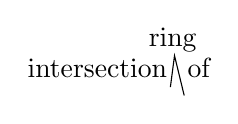
\begin{tikzpicture}[baseline=(base.base)]
\node[inner sep=0] (base) {intersection};
\node[anchor=base west,inner sep=0,xshift=.7em] (right) at (base.base east) {of};
\node[anchor=south west,inner sep=0,xshift=-.7em,yshift=.5ex] (added) at (base.north east) {\inserted{\handwritten{ring}}};
\draw ([xshift=.1em,yshift=-.8ex]base.south east) -- ([xshift=.25em,yshift=.2ex]base.north east) -- ([xshift=.6em,yshift=-1.5ex]base.south east);
\end{tikzpicture}} cycles \mbox{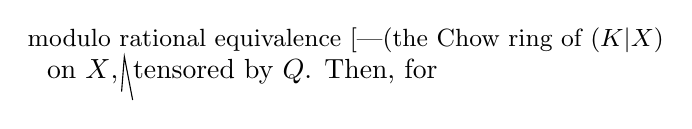
\begin{tikzpicture}[baseline=(base.base)]
\node[inner sep=0] (base) {on $X$,};
\node[anchor=base west,inner sep=0,xshift=.5em] (right) at (base.base east) {tensored by $Q$. Then, for};
\node[anchor=south west,inner sep=0,xshift=-.7em,yshift=.5ex,font=\small] at (base.north west) {\inserted{\handwritten{modulo rational equivalence \unsure{[|(}the Chow ring of $(\unsure{K|X})$}}};
\draw ([xshift=.1em,yshift=-.6ex]base.south east) -- ([xshift=.2em,yshift=.2ex]base.north east) -- ([xshift=.5em,yshift=-1.3ex]base.south east);
\end{tikzpicture}} each $i\handwritten{\leqslant}n$, we define a homomorphism
\[
\handwritten{\rho_X:C^i(X)\longrightarrow H_\ell^{2i}(X)}
\]
as follows. Let $Z$ be an irreducible subscheme of codimension $i$. The l-adic Poincare duality theorem asserts that the cup-product pairing
\[
\handwritten{H_\ell^j(X)\times H_\ell^{2n-j}(X)\longrightarrow H_\ell^{2n}(X)\overset{\unsure{\kappa_X|K_X}}{\overset{\sim}{\longrightarrow}}Q_\ell\quad(j=0,\ldotp\,\unsure{\ldotp}\,\ldotp,2n)}
\]
is a perfect duality of finite dimensional vector spaces, and so the element $\handwritten{\rho_X(Z)\in H_\ell^{2i}(X)}$ is uniquely determined by the condition
\[
\handwritten{\unsure{\kappa_X|K_X}\bigl(\alpha\cdot\rho_X(Z)\bigr)=\unsure{\kappa_Z|K_Z}\bigl(\operatorname{res}_Z(\alpha)\bigr)\quad\text{for all }\alpha\in H_\ell^{2n-2i}(X).}
\]

We then extend $\handwritten{\rho_X}$ to all of $C^{\handwritten{i}}(X)$ by linearity. Further, this homomorphism takes intersection product into cup-product, and thus it extends to a homomorphism of \handwritten{``}algebras\handwritten{''} \mbox{
\begin{tikzpicture}[baseline=(old.base)]
\node[inner sep=0] (old) {\deleted{on}};
\node[anchor=south west,inner sep=0,yshift=.2ex] at (old.north west) {\inserted{\handwritten{over}}};
\end{tikzpicture}} $Q$\unsure{.}
\[
\handwritten{\rho_X:C^*(X)\longrightarrow H_\ell^*(X)..}
\]

The image of a cycle under this homomorphism .is called the \uline{cohomology class} associated with th\rlap{\unsure{a|e}}et cycle, and we den\unsure{ö|o}te \unsure{f} $\handwritten{\rho_X}(C^{\mbox{\begin{tikzpicture}[baseline=(star.base)]
\node[inner sep=0] (star) {$\scriptstyle *$};
\node[anchor=base,inner sep=0,xshift=.12em,yshift=.35ex] at (star.base) {$\scriptstyle\handwritten{\unsure{\imath}}$};
\end{tikzpicture}}}(X))$ by $C_{\handwritten{\ell}}^*(X)$. A cycle is defined to be $Q_{\handwritten{\ell}}$-cohomologically equivalent to $0$ if it is in the kernel of the homomorphism $\handwritten{\rho_X.}$
